% !TeX root = main.tex


\begin{savequote}[70mm]
,,''
\qauthor{}
\end{savequote}

\chapter{Metody pozyskiwania trójwymiarowego obrazu sceny}
\label{chap:porownanie}

Metody pozyskiwania trójwymiarowego obrazu sceny można podzielić ze względu
na wykorzystywane do tego celu urządzenia. W porównaniu skupiono się na praktycznych
cechach przedstawionych rozwiązań, ponieważ ostatecznie wykorzystywane będą gotowe
algorytmy, ich implementacja nie jest celem tej pracy.


\section{Stereowizja}

Stereowizja jest techniką obrazowania opierającą się na analizie obrazów wielu
(najczęściej dwóch) kamer. Algorytmy bazują na dysparacji, czyli względnej odległości pomiędzy
obrazami tego samego punktu w różnych kamerach, można w nich wydzielić 3 kroki:

\begin{enumerate}
\item detekcja punktów charakterystycznych
\item dopasowanie odpowiedników
\item rekonstrukcja współrzędnych 3D
\end{enumerate}

Dodatkowo konieczne jest wstępne przetworzenie obrazów tak, aby przedstawiały
one widok w taki sposób, jakby płaszczyzny obrazowania kamer były równoległe
(proces ten zwany jest rektyfikacją obrazu). W tym celu konieczna jest wstępna
kalibracja układu kamer, dająca w wyniku położenie kamer względem siebie (przesunięcie
oraz obrót), a także wyliczająca parametry wewnętrzne każdej z kamer (zniekształcenia
wnoszone przez soczewki obiektywu). Proces kalibracji przeprowadza się raz dla danego
położenia kamer, po każdorazowej zmianie ich pozycji konieczna jest powtórna kalibracja.

\subsection{Wymagania sprzętowe}
Najważniejszym elementem przy stereowizji są kamery -- uzyskane rezultaty zależą
bezpośrednio od ich jakości. Stosowanie kamer z interfejsem analogowym jest możliwe, jednak nie
jest zalecane przy dynamicznych scenach. Obiekty poruszające się z dużą szybkością
są wykrywane błędnie bądź całkowicie ignorowane ze względu na występujące rozmycie
wynikające ze stosowania przeplotu podczas akwizycji z kamer analogowych. Najlepsze wyniki
uzyskuje się stosując dobrej jakości kamery z interfejsami cyfrowymi, jednak ich
koszt jest dużo wyższy.

Samo rozmieszczenie kamer również ma istotny wpływ na uzyskiwane wyniki -- kamery
umieszczone blisko siebie będą dawały dobre wyniki dla obiektów znajdujących się
blisko nich, kamery rozmieszczone szerzej pozwalają na uzyskanie lepszej rozdzielczości
dla obiektów znajdujących się daleko kosztem częściowej bądź całkowitej utraty
informacji o obiektach bliskich. Od rozdzielczości kamery zależy uzyskiwana rozdzielczość
przy rekonstrukcji sceny 3D, jednak wraz z jej wzrostem rośnie czas wymagany do
przetworzenia pojedynczej klatki obrazu.

Problemem możę być samo mechaniczne mocowanie kamer.
Musi być ono wykonane bardzo solidnie, gdyż w przypadku nawet małej zmiany orientacji
kamer względem siebiewymagana jest ponowna kalibracja całego systemu. Aby pozbyć
się tej wady można stosować zintegrowane moduły zawierające dwie (bądź więcej)
kamery w jednej obudowie, to jednak uniemożliwia eksperymentowanie z odległością
kamer od siebie.

\subsection{Złożoność obliczeń}

\cite{4670774} \cite{Hirschmuller:2008:SPS:1340087.1340245}

Przy wykorzystaniu programowej wersji algorytmów stereowizyjnych działających
na przeciętnym komputerze domowym, można osiągnąć wydajność od kilku do kilkunastu
klatek na sekundę. W związku z tym rozwiązania programowe
nie nadają się do wykorzystania w środowisku, które ulega częstym i dynamicznym
zmianom (a takie jest otoczenie robota mobilnego).

Dużo lepiej sprawdzają się rozwiązania sprzętowe, w których algorytm tworzenia
mapy dysparacji zaimplementowany jest w układach FPGA zintegrowanych w jednym
module z kamerami. W tym przypadku wydajność jest stała i niezależna od platformy,
na której uruchomione będą algorytmy sterowania robota, i wynosi (w zależności
od producenta) od kilkunastu do ponad 30 FPS. Największą wadą takiego rozwiązania
jest jego koszt -- wynoszący od kilkuset do kilku tysięcy dolarów. Dla porównania
dwie kamery analogowe można kupić za ok. 200\$.

\subsection{Problemy związane z algorytmem}

Algorytm opiera się o wykrywanie punktów charakterystycznych w obrazie, a to najczęściej
sprowadza się do analizy obrazu krawędziowego. W związku z tym obiekty o jednolitej,
drobnej teksturze (bądź całkowicie gładkie) są słabo bądź całkowicie niewykrywalne.
W najlepszym wypadku wykrywane są jedynie ich krawędzie, co prowadzi do powstawania
dużych, niezidentyfikowanych obszarów w obrazie (rysunek XX przedstawia taką sytuację).

Jednym z rozwiązań tego problemu może być zastosowanie dodatkowego projektora
wyświetlającego specjalnie przygotowany wzór (\cite{konolige-icra-2010-a}) w celu
pokrycia obiektów sztuczną teksturą umożliwiającą poprawę wyników stereowizji.
Drugą możlwością poprawy sytuacji jest stosowanie dodatkowego etapu przetwarzania
obrazu po wygenerowaniu wstępnej mapy głębokości. Po segmentacji obrazu na podstawie
koloru wybierane są obszary jednolite, a następnie w mapie głębi wypełniane są
interpolowanymi wartościami z ich krawędzi.

Oba rozwiązania dają dobre rezultaty, jednak komplikują bądź budowę urządzenia,
bądź wprowadzają dodatkowy narzut obliczeniowy.

\subsection{Pomiary}

W celu sprawdzenia w praktyce jakie rezultaty można osiągnąć na dostępnym sprzęcie
przygotowano prosty układ pomiarowy i zebrano kilka pomiarów dla różnych scen.
Para stereowizyjna została złożona z dwóch kamer firmy Ganz, model ZC-NAF27, które
ustawione zostały w taki sposób, aby ich osie optyczne były możliwie równoległe,
a ich odległość wynosiła 12cm (podytkowane właściwościami mechanicznymi platformy,
na której zostały zamontowane). Po kalibracji obu kamer uruchomiono algorytm
dopasowania i generacji mapy dysparacji (wykorzystujący bibliotekę OpenCV) na
komputerze wyposażonym w procesor Intel Core2Duo E6550 2.33GHz oraz 4GB pamięci
RAM, pracującym pod kontrolą systemu Ubuntu 10.04. Wygenerowanie pojedynczej mapy
głębi zajmowało ok. 130ms (7.7 klatki na sekundę).

Poniżej przedstawione są wygenerowane mapy głębi nałożone na obraz z którego powstały
(dokładnie na obraz z lewej kamery, ponieważ w jej układzie mapa ta jest wyliczana).
Przedstawione są trzy sceny przedstawiające charakterystyczne cechy tej metody
pozyskiwania informacji o głebi. Scena przedstawiona na rysunku~\ref{fig:stereo_1}
zawiera dwie jednakowe przeszkody umieszczone w różnej odległości przed robotem.
Algorytm dobrze wykrywa krawędzie przeszkód, jednak na ich powierzchni oznaczane
są jedynie miejsca, gdzie naniesione są napisy i rysunki. W niektórych miejscach
widać błędne dopasowania punktów charakterystycznych (widoczne jako plama w kolorze
znacznie odbiegającym od otoczenia, np. na dole prawego pudełka). Szary kolor na
mapie głębi oznacza piksele niezidentyfikowane. Kolor piksela oznacza jego odległość
od kamery, najbliższe są czerwone, najdalsze są niebieskie.

\begin{figure}[h!]
\centering
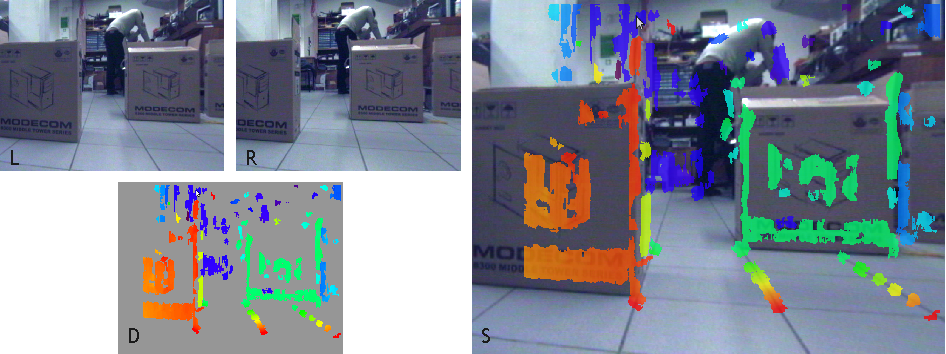
\includegraphics{../img/stereo_1}
\caption[Pierwsza scena testowa stereowizji]{Pierwsza scena testowa stereowizji. L i R to obraz odpowiednio z~lewej i~prawej kamery, D~przedstawia mapę głębi, S~przedstawia mapę głębi nałożoną na obraz z~lewej kamery.}
\label{fig:stereo_1}
\end{figure}

Scena na rysunku~\ref{fig:stereo_2} zawiera przeszkody pokryte bardziej zróżnicowaną
teksturą, dzięki czemu są one znacznie lepiej wykrywane, a mapa głębi jest bardziej
wypełniona.

Ostatni eksperyment (rysunek~\ref{fig:stereo_3}) miał na celu pokazanie problemu
przy wykrywaniu dużych, jednolitych obiektów. Tablica zajmuje dużą część obrazu
i stanowi poważną przeszkodę dla robota. Na mapie głębi jednak oznaczone są jedynie
jej boczne krawędzie, co mogłoby doprowadzić do próby przejazdu pomiędzy nimi.

\begin{figure}[h!]
\centering
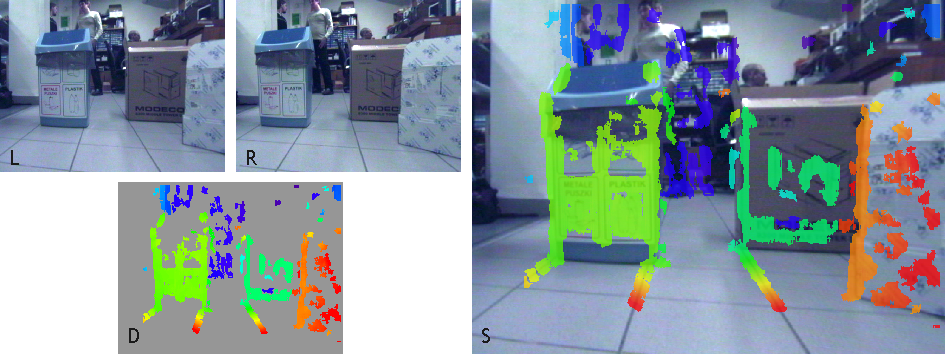
\includegraphics{../img/stereo_2}
\caption[Druga scena testowa stereowizji]{Druga scena testowa stereowizji zawierająca obiekty o zróżnicowanej teksturze. L i R to obraz odpowiednio z lewej i prawej kamery, D przedstawia mapę głębi, S przedstawia mapę głębi nałożoną na obraz z lewej kamery.}
\label{fig:stereo_2}
\end{figure}

\begin{figure}[h!]
\centering
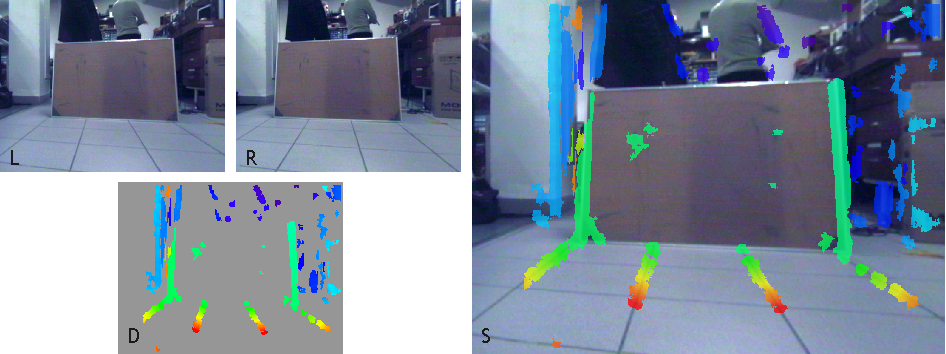
\includegraphics{../img/stereo_3}
\caption[Trzecia scena testowa stereowizji]{Trzecia scena testowa stereowizji pokazująca problemy z dużymi, jednolitymi przeszkodami. L i R to obraz odpowiednio z lewej i prawej kamery, D przedstawia mapę głębi, S przedstawia mapę głębi nałożoną na obraz z lewej kamery.}
\label{fig:stereo_3}
\end{figure}

Niewątpliwą zaletą stereowizji w porównaniu do innych metod jest

\section{Światło strukturalne}

Inną metodą pomiaru i odtwarzania informacji i głębi sceny bazującą na analizie
obrazu jest wykorzystanie światła strukturalnego. Na scenę rzucane jest światło
formujące znany wzór, a kamera umieszczona jest w taki sposób, aby obserwować
scenę pod innym kątem niż orientacja rzutnika. Na podstawie odczytanej deformacji
wzorca prz użyciu algorytmów bazujących na riangulacji wyliczane są rzeczywiste
współrzędne punktów w obrazie. Rzucane mogą być różne wzory, od pojedynczej linii
przesuwającej się po scenie (w takim przypadku scena jest analizowana stopniowo),
przez siatki punktów bądź linii (cała scena oświetlana jednocześnie) aż do złożenia
wielu siatek o zróżnicowanej gęstości wyświetlanych sekwencyjnie (korzystając
na przykład z kodu Graya można dokładniej określić, do której części wzorca należą
obserwowane punkty).

\subsection{Rozwiązania programowe i sprzętowe}

W przypadku stosowaniaalgorytmów zaimplementowanych programowo uruchamianych na
komputerze sterującym można wymienić praktycznie takie same wady, jak przy stereowizji.
Największą z nich jest obciążenie systemu, gdyż algorytm jest dość skomplikowany.

Rozwiązania sprzętowe rozwiązują problem szybkości działania i obciążenia
komputera sterującego, jednak ich cena przez bardzo długi czas była wysoka
(rzędu setek do tysięcy dolarów). Pod koniec 2010 roku pojawiło się jednak urządzenie
o cenie o rząd wielkości niższej, będące faktycznie sprzętowym sensorem głębi
opartym o analizę światła strukturalnego. Niską cenę zawdzięcza masowej produkcji
-- jest produkowany jako kontroler do gier, i jako taki ma zdecydowanie większy
rynek zbytu niż tradycyjne, specjalizowane rozwiązania. Jego dokładniejszy opis
znajduje się w kolejnej sekcji.

\section{Microsoft Kinect}

Jest to kontroler do gier dla konsoli Xbox wykorzystujący analizę światłą strukturalnego.
Pomimo jego pierwotnego przeznaczenia, kilka dni po premierze został opublikowany
nieoficjalny sterownik umożliwiający wykorzystanie informacji z jego czujników na
komputerze PC. Jego niska cena (500PLN), dostępność wielu algorytmów ułatwiających
wykorzystanie dostarczanych przez niego informacji oraz szybkość i dokładność
działania sprawiły, że został on wybrany jako główne źródło informacji o scenie
do wykorzystania w projekcie.

\begin{figure}[h!]
\centering
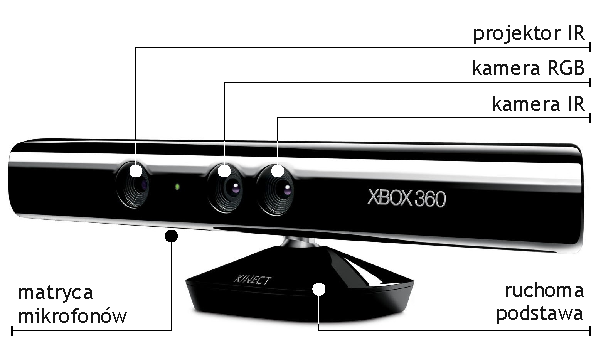
\includegraphics{../img/kinect_hardware}
\caption[Sensor Kinect firmy Microsoft]{Sensor Kinect firmy Microsoft z zaznaczonymi
kluczowymi elementami.}
\label{fig:kinect_hardware}
\end{figure}

\subsection{Budowa}

Kluczowe elementy sensora Kinect zaznaczone są na rysunku~\ref{fig:kinect_hardware}.
Pomiar głębi realizowany jest przy użyciu pary złożonej z projektora podczerwieni
oraz kamery rejestrującej obraz w tym paśmie. Kamera RGB umieszczona pomiędzy nimi
służy do rejestracji widocznej sceny, a dzięki jej kalibracji z pomiarem głębi
możliwe jest tworzenie trójwymiarowych map otoczenia z nałożoną teksturą (dane
kalibracyjne dostarczone przez producenta są zapisane bezpośrednio w urządzeniu).

Dodatkowo Kinect wyposazony jest w matrycę czterech mikrofonów, które mogą być
wykorzystane do lokalizacji źródeł dźwięku w przestrzeni, a~także podstawę umożliwiającą
pochylanie sensora w~zakresie~27\textdegree~w~górę i~w~dół.

Istotne parametry techniczne zebrane są w tabeli~\ref{tab:kinect_params}.

\begin{table}[h!]
\caption{Kinect -- parametry techniczne}
\centering
\begin{tabular}{lr}
\toprule
\textbf{Pole widzenia}\\
\midrule
Poziome & 57\textdegree \\
Pionowe & 43\textdegree \\
Zakres ruchu góra/dół & $\pm$27\textdegree \\
Efektywny pomiar odległości & 1.2m - 3.5m \\
\midrule
\textbf{Kamera RGB} \\
\midrule
Rozdzielczość & 640x480px \\
Głębia bitowa & 8 bitów \\
Prędkość & 30kl/s \\
\midrule
\textbf{Mapa głębi} \\
\midrule
Rozdzielczość & 320x240px \\
Głębia bitowa & 16 bitów \\
Prędkość & 30kl/s \\
\bottomrule
\end{tabular}
\label{tab:kinect_params}
\end{table}

\subsection{Działanie}

Sercem urządzenia jest dedykowany układ tworzący mapę głębi na podstawie analizy
obrazu z kamery IR. W pierwszym kroku na scenę rzucany jest specjalny wzór
(przedstawiony na rysunku~\ref{fig:kinect_pattern}), a uzyskany obraz jest rejestrowany.

\begin{figure}[h!]
\centering
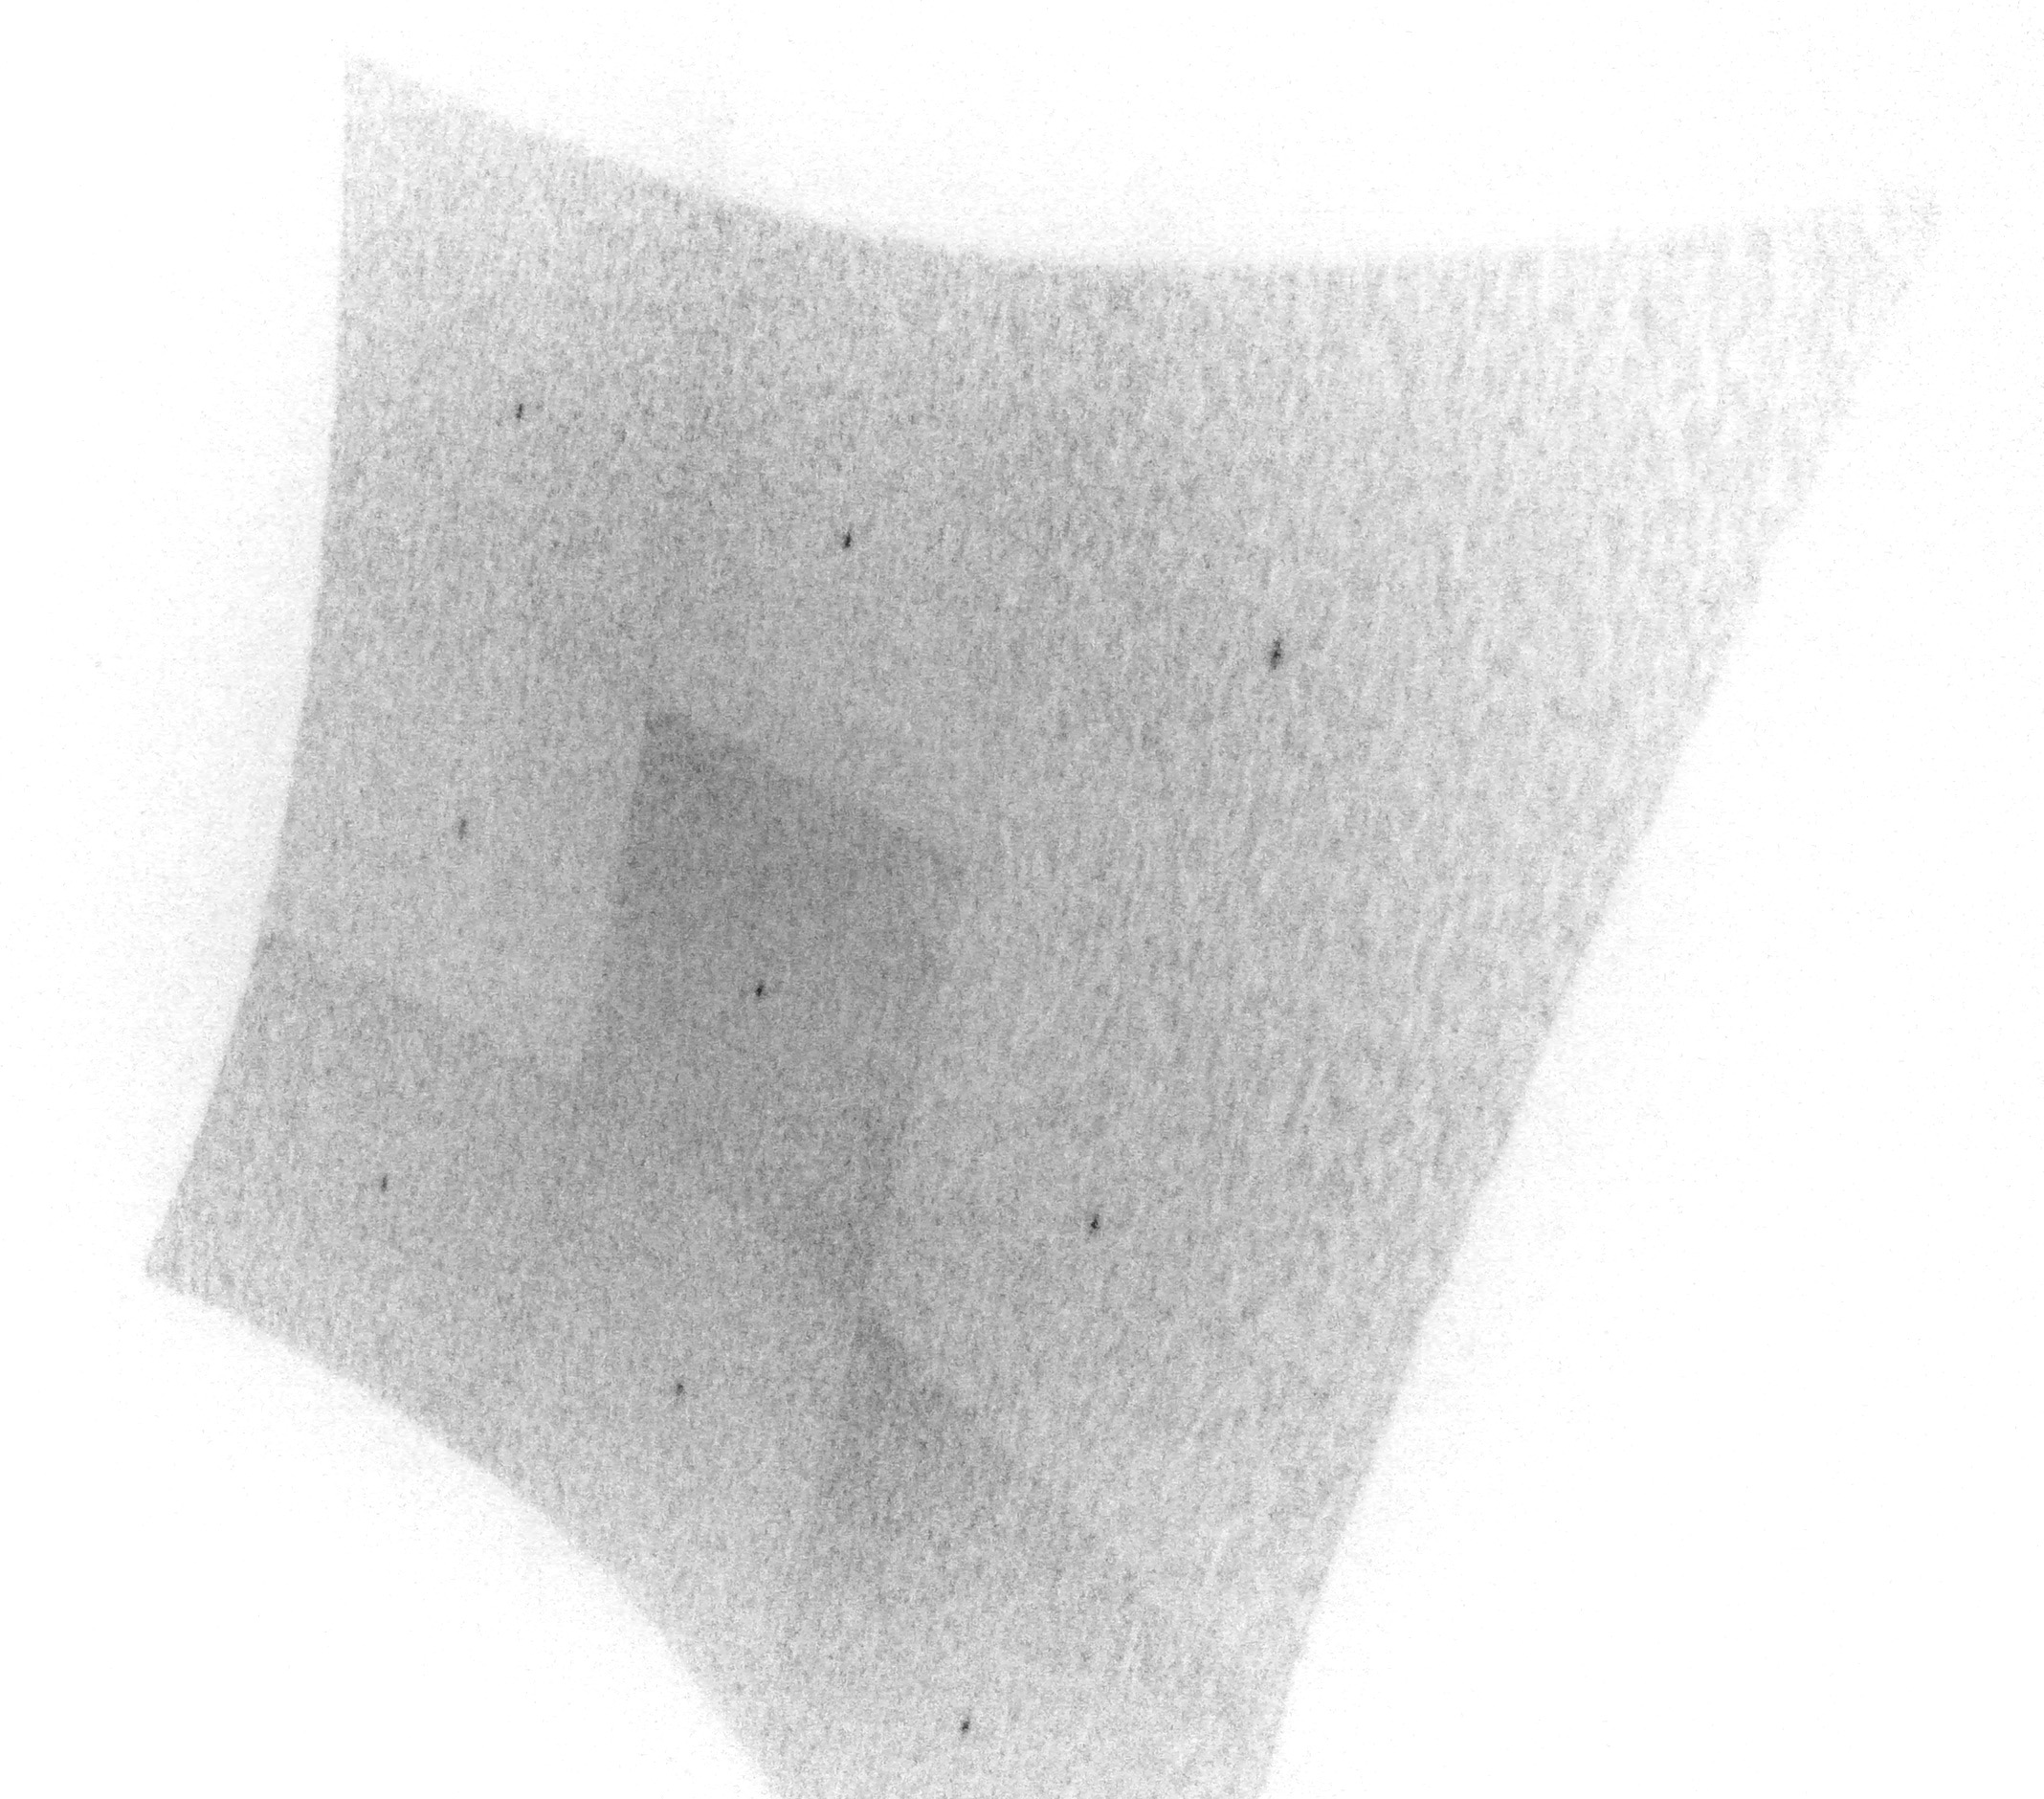
\includegraphics[width=8cm]{../img/kinect_pattern}
\caption[Wzór rzucany przez Kinect]{Wzór rzucany przez Kinect (kolory odwrócone,
ciemny punkty oznaczają miejsca oświetlane przez rzutnik podczerwieni). Źródło:
http://www.anandtech.com/show/4057/microsoft-kinect-the-anandtech-review/2}
\label{fig:kinect_pattern}
\end{figure}

Wzór ma specjalną strukturę, umożliwiającą poprawne zlokalizowanie analizowanych
pikseli w obrazie wzorcowym bez konieczności wielokrotnego rzutowania różnych
tekstur (tak jak przy metodzie wykorzystującej kod Graya i coraz węższe paski).
Zaczynając od największych bloków wyróżnić w nim można szachownicę 3x3 pola, a na
środku każdego z nich jaśniejszy punkt służący do lokalizacji centrum danego segmentu.
KAżde z pól pokryte jest siatką punktów ułożonych w taki sposób, aby ich bloki
potwarzały się bardzo rzadko lub wcale w obrębie danego pola szachownicy (w ten
sposób wyeliminowany został problem fałszywych dopasować podczas porównywania
z obrazem referencyjnym). Po zlokalizowaniu pozycji pikseli w mapie wzorcowej
z triangulacji wyliczane jest ich względne przesunięcie, a z niego ostateczna
mapa głębi.

\subsection{Pomiary}

Celem pomiarów było porównanie działania sensora Kinect i pary stereowizyjnej.
W tym celu przeanalizowano te same sceny, a obrazy wynikowe przedstawione są
poniżej. Największą różnicę widać w pokryciu obrazu na mapie głębi (w przypadku
Kinecta fragmenty nierozpoznane oznaczane są na czarno). Drugą różnicą, której
nie widać na obrazkach, jest prędkość działania. Jako, że w przypadku sensora
firmy Microsoft algorytm jest zaimplementowany sprzętowo, co ma dwie zalety:
po pierwsze system komputera sterującego jest mniej obciążony, po drugie niezależnie
od jego obciążenia akwizycja danych działa z prędkością 30 klatek na sekundę.

\begin{figure}[h!]
\centering
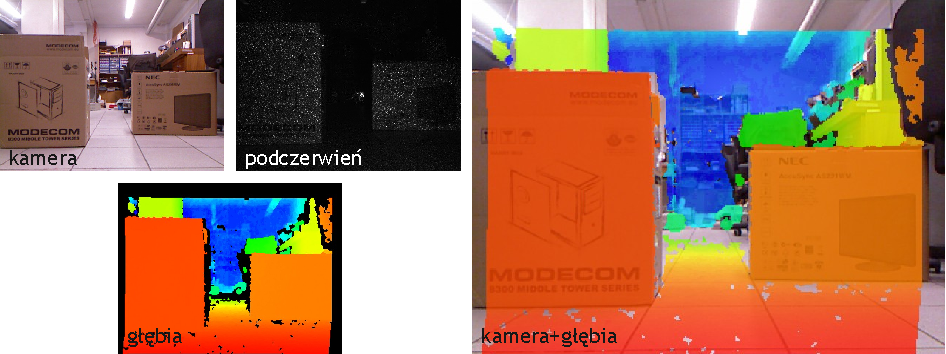
\includegraphics{../img/kinect_1}
\caption[Kinect -- pierwsza scena testowa]{Kinect -- pierwsza scena testowa}
\label{fig:kinect_1}
\end{figure}

Na rysunkach pokazany jest obraz z kamery RGB orazbraz widziany przez sensor
podczerwieni. Mapa głębi wyliczona na podstawie tego obrazu jest dodatkowo nakładana
na obraz RGB aby pokazać, w jaki sposób punkty z mapy głebi są skalibrowane z obrazem RGB.
Ogólnie dane dostarczane przez ten sensor są dużo lepszej jakości niż uzyskiwane
ze stereowizji, jednak istnieją przypadki trudne. Jednym z nich jest wykrywanie
wąskich, ciemnych przedmiotów (takich jak nogi od krzesła widoczne na
rysunku~\ref{fig:kinect_3}). Obiekty takie są zbyt małe, aby ich pokrycie przez
wzór referencyjny było odpowiednio duże, dodatkowo czarny kolor w dużym stopniu
pochłania światło podczerwone dodatkowo utrudniając ich lokalizację. W przypadku
korzystania ze stereowizji podobne przypadki nie stanowią problemu, ponieważ
wąskie, wyraźnie widoczne linie w obrazie są wykrywane jako punkty charakterystyczne
i są wykorzystywane w procesie tworzenia mapy dysparycji (można to zaobserwować
na rysunku~\ref{fig:stereo_3}, gdzie pomimo słabego wykrywania całej powierzchni
podłogi doskonale zaznaczane są czarne linie fug pomiędzy płytkami).

\begin{figure}[h!]
\centering
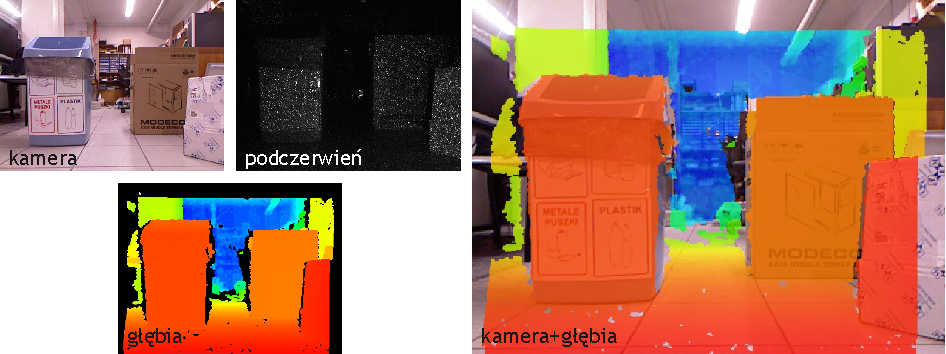
\includegraphics{../img/kinect_2}
\caption[Kinect -- druga scena testowa]{Kinect -- druga scena testowa}
\label{fig:kinect_2}
\end{figure}

\begin{figure}[h!]
\centering
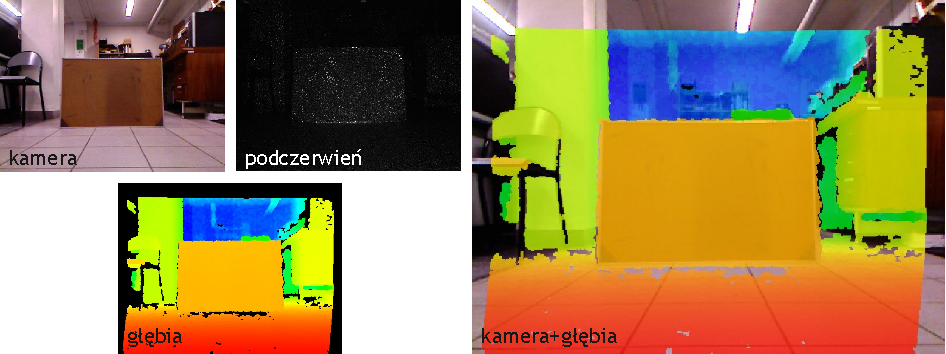
\includegraphics{../img/kinect_3}
\caption[Kinect -- trzecia scena testowa]{Kinect -- trzecia scena testowa}
\label{fig:kinect_3}
\end{figure}

\section{Pomiar czas przelotu wiązki światła}

Kamery TOF\footnote{z ang. {\it time-of-flight}, czas przelotu} działają na zasadzie
pomiaru czasu przelotu wiązki światła od generatora do kamery po jego odbiciu od
obiektów. Działanie to jest analogiczne do działania skanerów laserowych, z tą różnicą,
że w przypadku skanerów emitowana jest pojedyncza wiązka światła, natomiast kamery TOF
oświetlają i wykonują pomiar całej sceny naraz.

\subsection{Zalety i wady}

Kamery działające na zasadzie pomiaru czasu przelotu światła mają wiele zalet, spośród
których najważniejsze to:

\begin{itemize}
\item prostota konstrukcji -- cały system składa się z pojedynczego, zwartego
modułu zawierającego zarówno kamerę jak i oświetlacz,
\item szybkość działania -- dzięki naświetlaniu całej klatki jednocześnie oraz
biorąc pod uwagę prędkość światła, możliwe jest uzyskanie prędkości nawet 100 klatek
na sekundę,
\item niskie obciążenie systemu -- kamera zwraca obraz zawierający czas przelotu
światła, z którego w prosty sposób obliczyć można odległość, w przeciwieństwie do
innych rozwiązań, gdzie wymagane jest stosowanie skomplikowanych algorytmów w celu
wyliczenia ostatecznej odległości do obiektów.
\end{itemize}

Własności te sprawiają, że kamery TOF wydają się być bardzo dobrym rozwiązaniem
do zastosowania przy nawigacji robota. Niestety, mają też kilka wad:

\begin{itemize}
\item cena -- jako że rozwiązania te są stosunkowo nowe a także bardzo skomplikowane
pod względem technicznym, ich cena jest wielokrotnie wyższa od układów opartych na
stereowizji lub świetle strukturalnym,
\item rozdzielczość -- obecnie produkowane sensory posiadają rozdzielczość maksymalną
rzędu 320x240px, a tańsze modele często posiadają rozdzielczość poniżej 100x100px,
\item wielokrotne odbicia -- jako, że cała scena naświetlana jest naświetlana jednocześnie,
może się zdarzyć, że światło odbite i rozproszone od bliskiego obiektu dotrze do
sensora wcześniej, niż światło odbite od właściwego punktu widzianego w tym miejscu
matrycym przez co niektóre pomiary mogą być zafałszowane,
\item oświetlenie otoczenia,
\item interferencja.
\end{itemize}
